\section{Figures} \label{sec:Figures}

\subsection*{Additional Market Surface Example}

To illustrate the stability of the empirical implied volatility surface across different sample periods, 
Figure~\ref{fig:MarketSurfaceApr2023} shows the S\&P~500 surface constructed from April 2023 option data. 
The same cleaning and interpolation procedures as described in Section~\ref{subsec:EmpiricalVolatilitySurface} 
were applied. The surface exhibits the same qualitative features as the March 2023 surface: convex volatility smiles, 
a negative and increasing ATM skew, and an approximate power-law decay in the skew term structure. 
This confirms that the stylized facts underlying the simulation quality criteria are consistently present 
in market data across different months.

\begin{figure}[H]
    \centering
    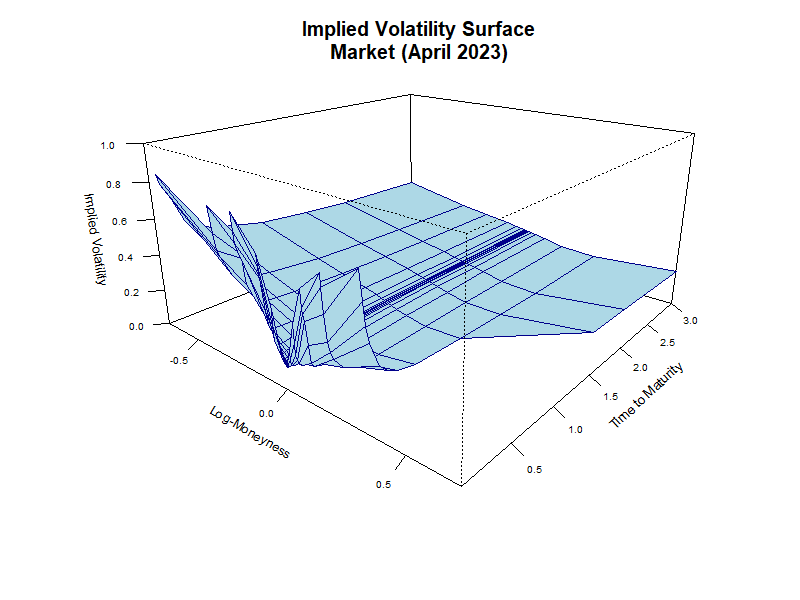
\includegraphics[width=0.45\textwidth]{figures/A.1 Market Surface/market_apr-23_iv_surface.png}
    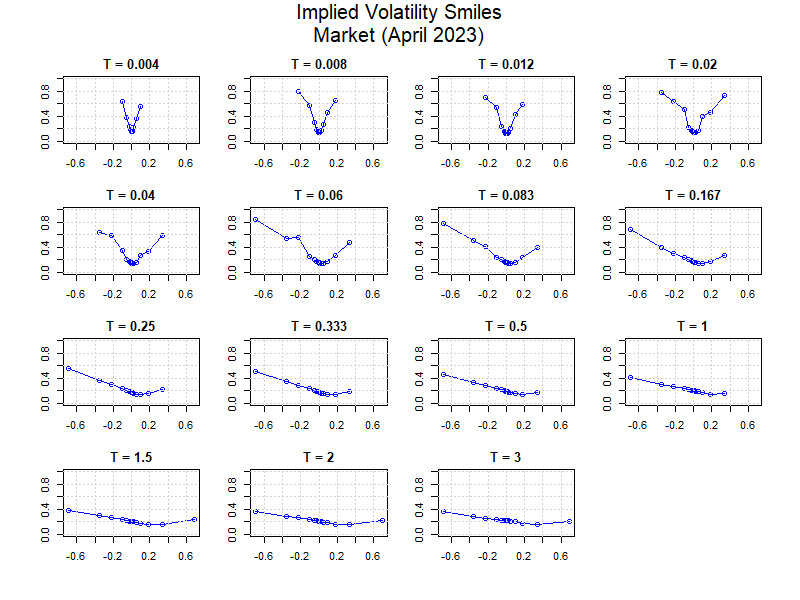
\includegraphics[width=0.45\textwidth]{figures/A.1 Market Surface/market_apr-23_iv_smiles.png}
    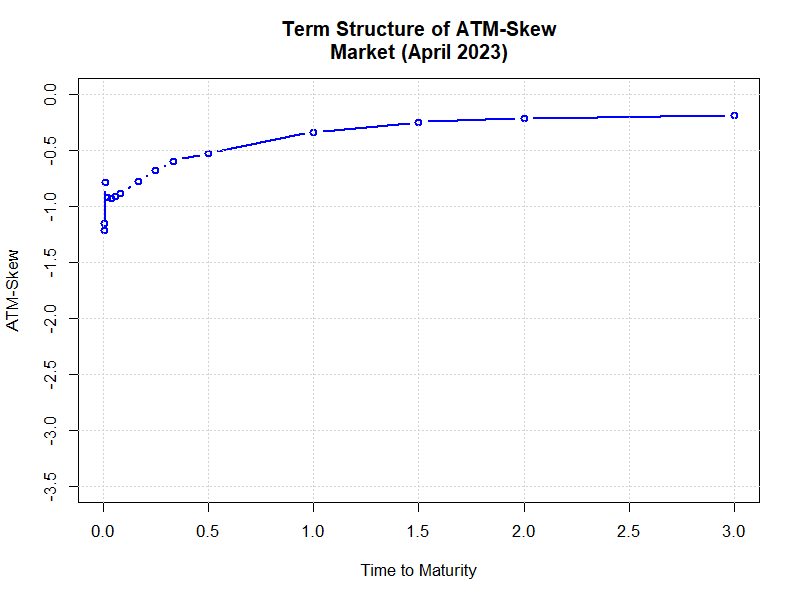
\includegraphics[width=0.45\textwidth]{figures/A.1 Market Surface/market_apr-23_atm_skew.png}
    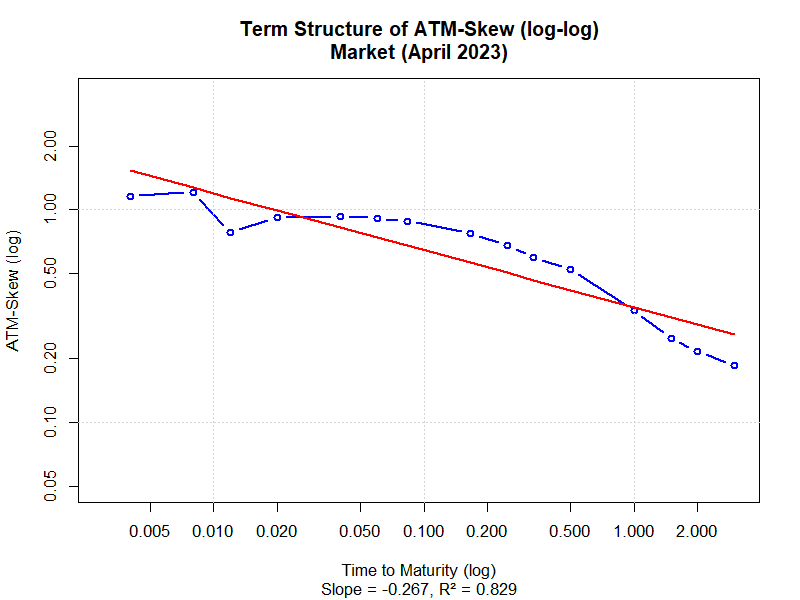
\includegraphics[width=0.45\textwidth]{figures/A.1 Market Surface/market_apr-23_atm_skew_log.png}
    \caption{Empirical implied volatility surface, volatility smiles, and ATM skew (S\&P~500; April 2023).}
    \label{fig:MarketSurfaceApr2023}
\end{figure}
